Setelah mempelajari berbagai teknologi dan \textit{library} yang relevan, tahap ini difokuskan pada evaluasi dan konfirmasi teknologi yang akan digunakan untuk mengimplementasikan fitur-fitur yang telah ditentukan dalam spesifikasi perangkat lunak. Penentuan teknologi ini dilakukan dengan mempertimbangkan hasil studi literatur, eksplorasi teknologi, serta diskusi bersama dosen pembimbing.

\begin{enumerate}[label*=\arabic*.,ref=\arabic*]
    \item \textbf{Fitur}\\
    Fitur yang akan diimplementasikan dalam perangkat lunak adalah sebagai berikut:
    \begin{enumerate}[label=\alph*.]
        \item \textbf{Pengelolaan Templat Website}\\
        Perangkat lunak menyediakan antarmuka berbasis REST API yang memungkinkan pengguna untuk mendefinisikan dan mengelola templat \textit{website} target.
        
        \item \textbf{\textit{Generate} Website}\\
        Perangkat lunak menyediakan antarmuka berbasis REST API yang memungkinkan pengguna untuk melakukan pemilihan templat \textit{website} dan melakukan \textit{generate} pada \textit{website} yang dipilih. \textit{Website} hasil \textit{generate} mendukung otentikasi pengguna melalui Google \textit{Single Sign-On} (SSO) berbasis protokol OAuth 2.0.
    
        \item \textbf{Sinkronisasi Data Antara Basis Data \textit{Website} Target dan Aplikasi Internal}\\
        Perangkat lunak memiliki fitur sinkronisasi otomatis yang menjaga konsistensi data antara basis data \textit{website} target dan basis data aplikasi internal. Validasi data adalah bagian penting dari proses ini untuk memastikan integritas dan akurasi data yang disinkronkan.
    \end{enumerate}

    
    \item \textbf{Diagram Use Case}\\
    Untuk menggambarkan interaksi pengguna dengan fitur-fitur yang telah dirancang, diagram \textit{use case} disusun seperti pada Gambar \ref{fig:usecase-diagram}.
    \begin{figure}[H]
        \centering
        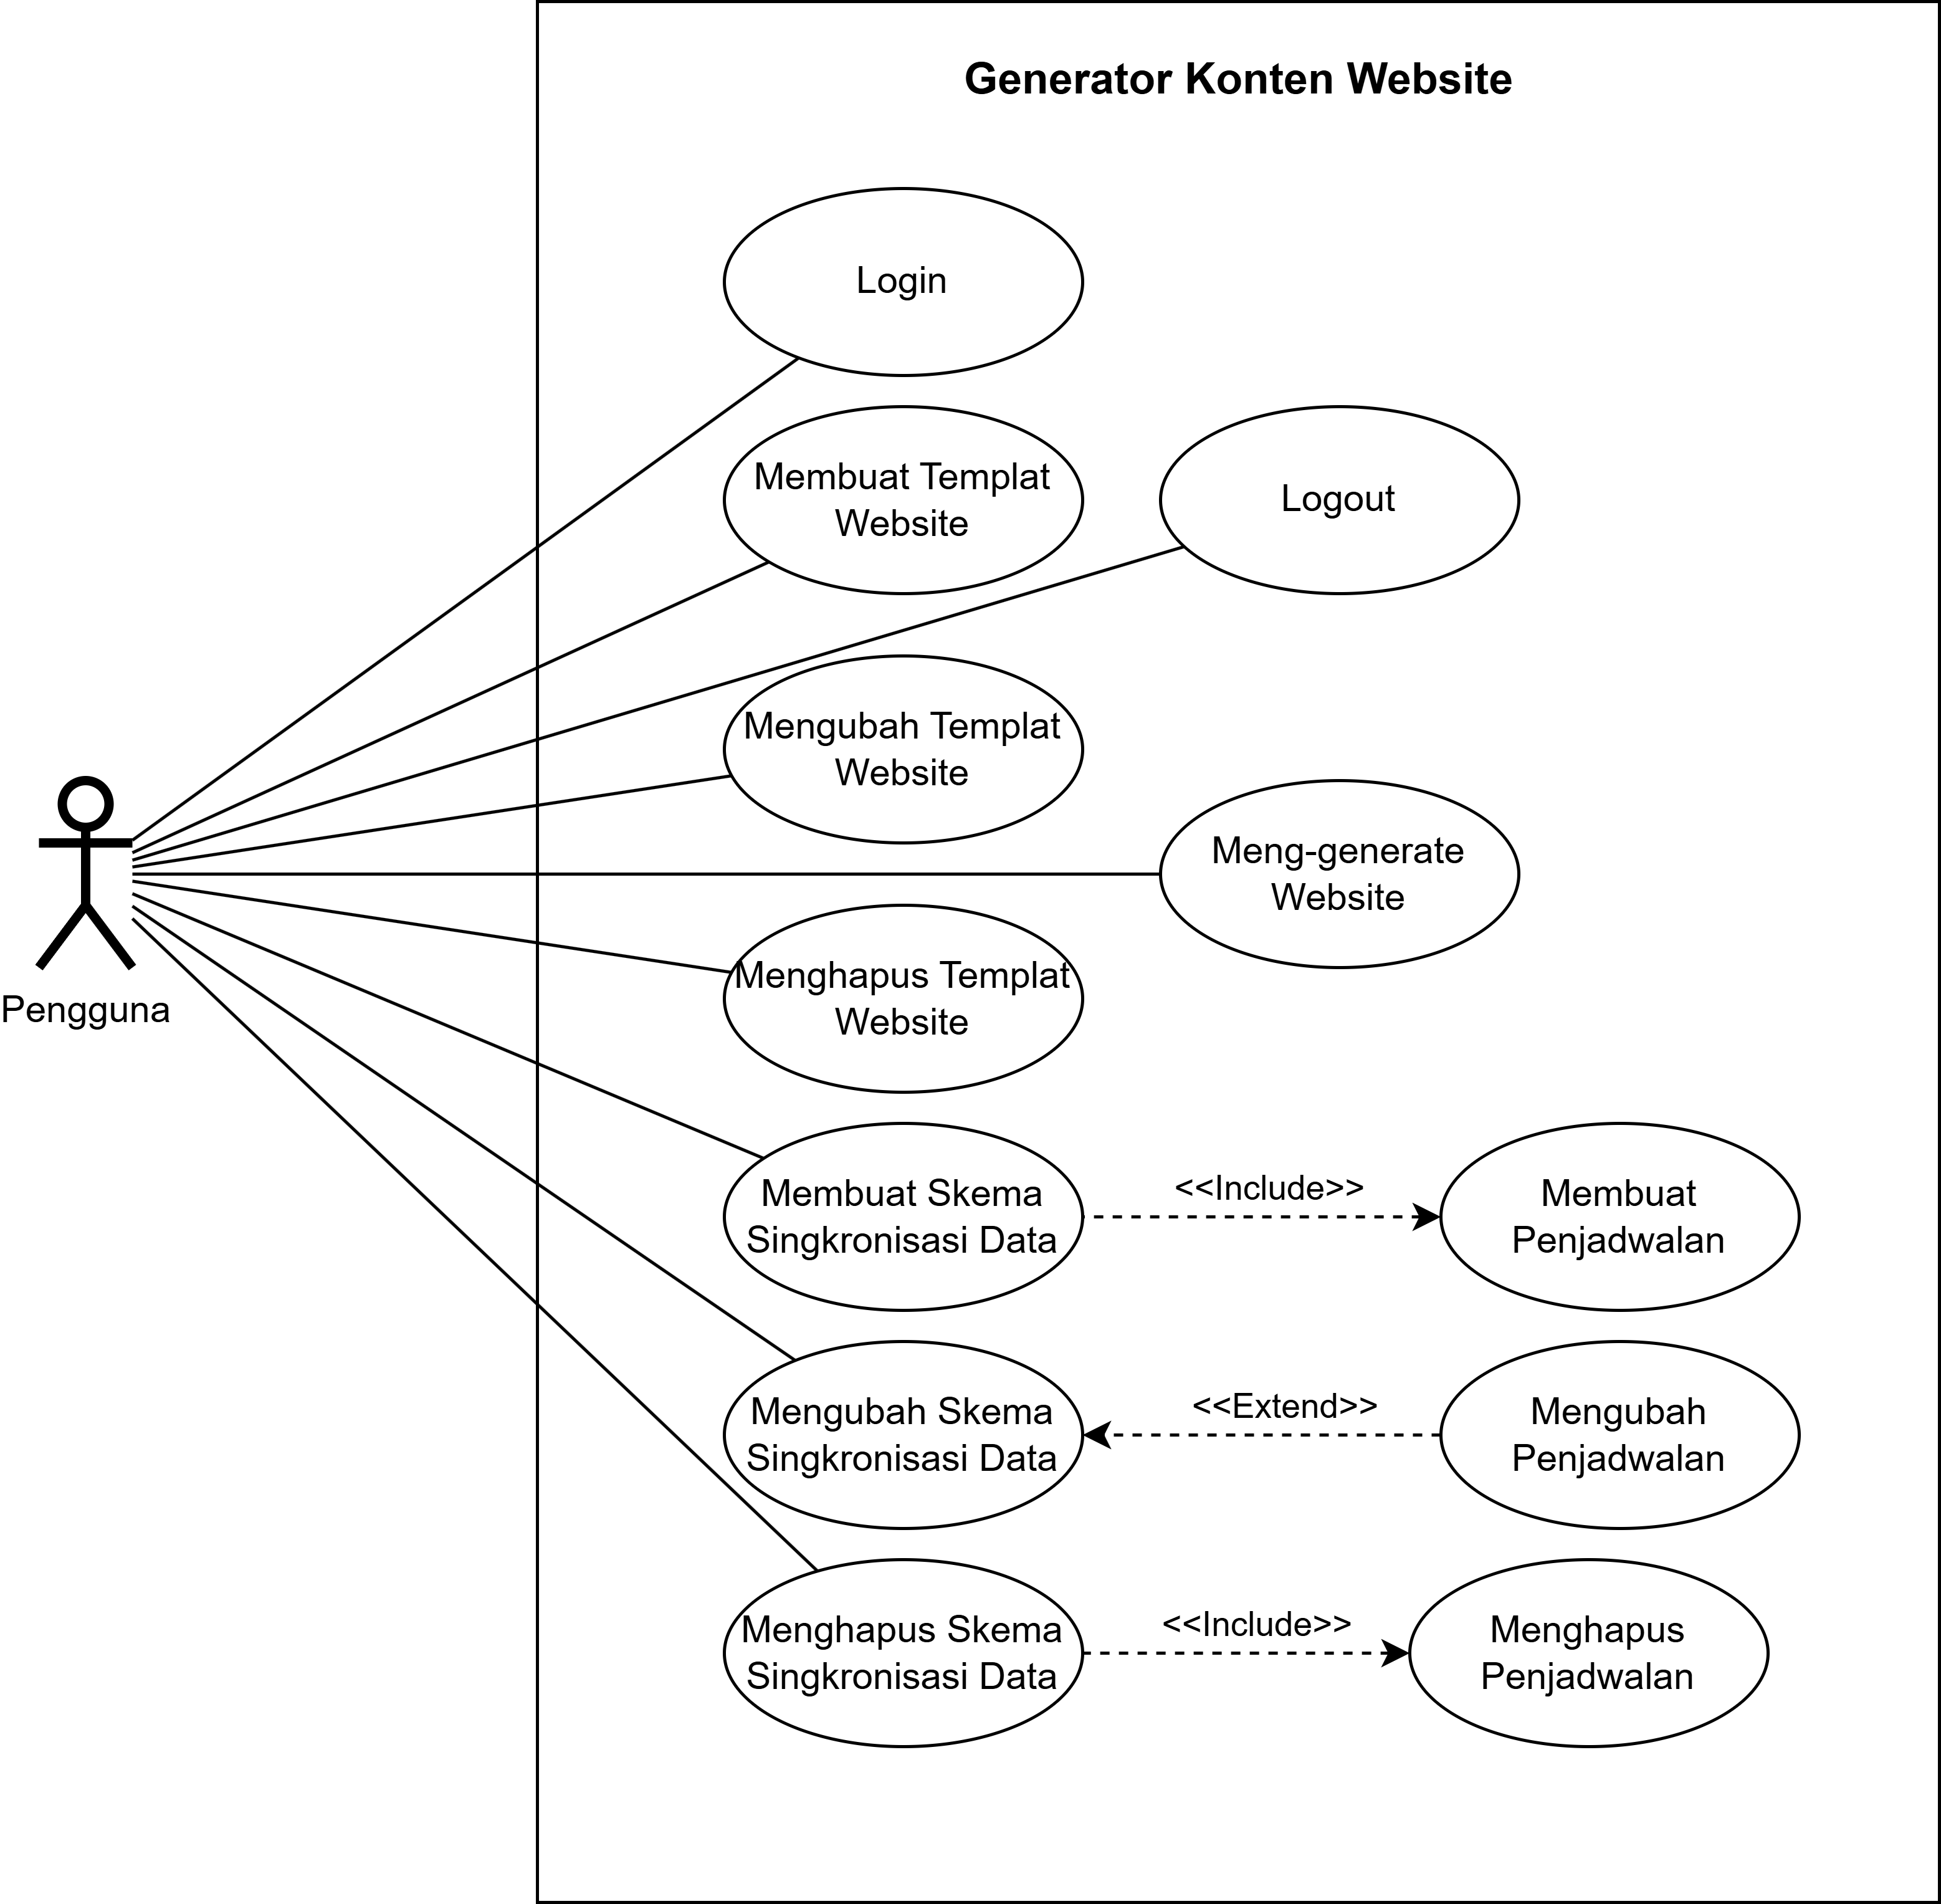
\includegraphics[width=0.8\linewidth]{figures/UseCaseDiagram.png}
        \caption{Diagram Use Case Generator Konten \textit{Website}}
        \label{fig:usecase-diagram}
    \end{figure}

    Diagram ini menunjukkan bahwa pengguna dapat melakukan berbagai tindakan, seperti mengelola templat, melakukan proses \textit{generate website}, mengatur sinkronisasi data, serta melakukan otentikasi.

    \item \textbf{Teknologi}\\
    Teknologi yang digunakan untuk mendukung implementasi fitur meliputi:
    \begin{enumerate}[label=\alph*.]
        \item \textbf{Bahasa Pemrograman}: JavaScript dengan \textit{runtime} Node.js.
        \item \textbf{Framework Backend}: Express.js untuk pengelolaan API dan server.
        \item \textbf{Library Backend}:
        \begin{itemize}
            \item \texttt{node-schedule}: Untuk penjadwalan sinkronisasi data.
            \item \texttt{joi}: Untuk validasi data.
            \item \texttt{sequelize}: Untuk manajemen basis data.
            \item \texttt{jsonwebtoken}: Untuk pengelolaan token otentikasi.
            \item \texttt{ejs}: Untuk pengelolaan templat halaman.
        \end{itemize}
        \item \textbf{Basis Data}: PostgreSQL untuk penyimpanan data yang terstruktur.
        \item \textbf{Frontend}: Dikembangkan menggunakan HTML, CSS, dan JavaScript tanpa menggunakan kerangka kerja (\textit{framework}).
        \item \textbf{Keamanan}: OAuth 2.0 Google untuk otentikasi dan kontrol akses pada aplikasi \textit{website}.
    \end{enumerate}
\end{enumerate}